\begin{figure}[t]
\centering
\resizebox{\textwidth}{!}{%
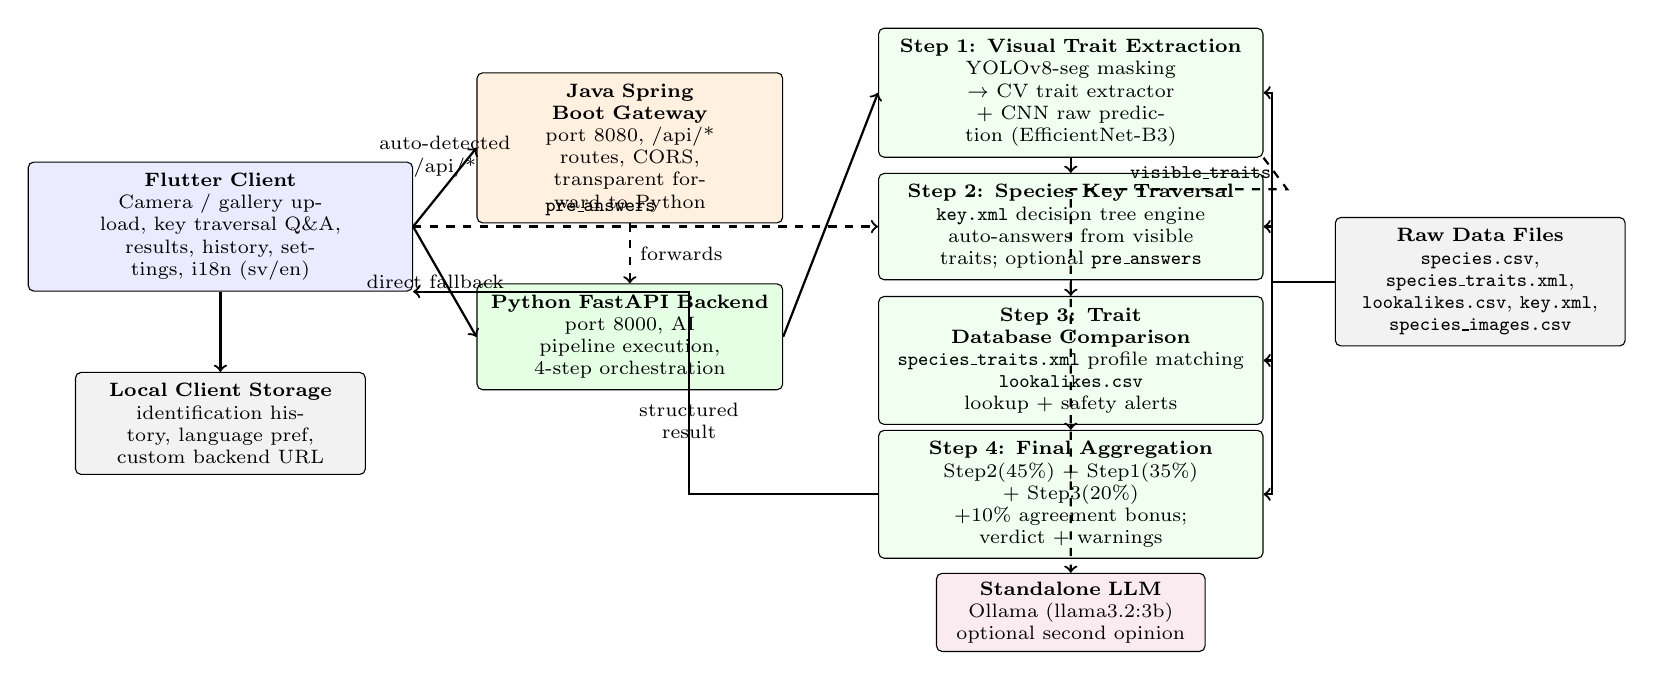
\begin{tikzpicture}[
    font=\scriptsize,
    box/.style={
        draw,
        rounded corners=2pt,
        align=center,
        minimum height=1.0cm,
        text width=3.6cm,
        inner sep=4pt
    },
    widebox/.style={
        draw,
        rounded corners=2pt,
        align=center,
        minimum height=1.0cm,
        text width=4.6cm,
        inner sep=4pt
    },
    smallbox/.style={
        draw,
        rounded corners=2pt,
        align=center,
        minimum height=0.8cm,
        text width=3.2cm,
        inner sep=3pt
    },
    data/.style={
        draw,
        rounded corners=2pt,
        align=center,
        minimum height=0.9cm,
        text width=3.4cm,
        inner sep=4pt,
        fill=gray!10
    },
    arrow/.style={->, thick},
    dasharrow/.style={->, thick, dashed},
    labelarrow/.style={->, thick, gray}
]

% ---------------------------------------------------------------------------
% Tier 1 — Client
% ---------------------------------------------------------------------------
\node[widebox, fill=blue!8] (client) at (0,0.3)
    {\textbf{Flutter Client}\\
    Camera / gallery upload, key traversal Q\&A,\\
    results, history, settings, i18n (sv/en)};

\node[data] (storage) at (0,-2.2)
    {\textbf{Local Client Storage}\\
    identification history, language pref,\\
    custom backend URL};

% ---------------------------------------------------------------------------
% Tier 2 — Backends
% ---------------------------------------------------------------------------
\node[box, fill=orange!12] (java) at (5.2,1.3)
    {\textbf{Java Spring Boot Gateway}\\
    port 8080, /api/* routes, CORS,\\
    transparent forward to Python};

\node[box, fill=green!10] (fastapi) at (5.2,-1.1)
    {\textbf{Python FastAPI Backend}\\
    port 8000, AI pipeline execution,\\
    4-step orchestration};

% ---------------------------------------------------------------------------
% Tier 3 — Pipeline Steps
% ---------------------------------------------------------------------------
\node[widebox, fill=green!6] (step1) at (10.8,2.0)
    {\textbf{Step 1: Visual Trait Extraction}\\
    YOLOv8-seg masking $\rightarrow$ CV trait extractor\\
    + CNN raw prediction (EfficientNet-B3)};

\node[widebox, fill=green!6] (step2) at (10.8,0.3)
    {\textbf{Step 2: Species Key Traversal}\\
    \texttt{key.xml} decision tree engine\\
    auto-answers from visible traits; optional \texttt{pre\_answers}};

\node[widebox, fill=green!6] (step3) at (10.8,-1.4)
    {\textbf{Step 3: Trait Database Comparison}\\
    \texttt{species\_traits.xml} profile matching\\
    \texttt{lookalikes.csv} lookup + safety alerts};

\node[widebox, fill=green!6] (step4) at (10.8,-3.1)
    {\textbf{Step 4: Final Aggregation}\\
    Step2(45\%) + Step1(35\%) + Step3(20\%)\\
    +10\% agreement bonus; verdict + warnings};

% ---------------------------------------------------------------------------
% Standalone LLM (optional consultation)
% ---------------------------------------------------------------------------
\node[smallbox, fill=purple!8] (llm) at (10.8,-4.6)
    {\textbf{Standalone LLM}\\
    Ollama (llama3.2:3b)\\
    optional second opinion};

% ---------------------------------------------------------------------------
% Tier 4 — Data
% ---------------------------------------------------------------------------
\node[data] (data) at (16.0,-0.4)
    {\textbf{Raw Data Files}\\
    \texttt{species.csv}, \texttt{species\_traits.xml},\\
    \texttt{lookalikes.csv}, \texttt{key.xml},\\
    \texttt{species\_images.csv}};

% ---------------------------------------------------------------------------
% Arrows — Client to Backends
% ---------------------------------------------------------------------------
\draw[arrow] (client.east) -- node[above, align=center] {auto-detected\\/api/*} (java.west);
\draw[arrow] (client.east) -- node[below, align=center, pos=0.35] {direct fallback} (fastapi.west);
\draw[arrow, dashed] (java.south) -- node[right] {forwards} (fastapi.north);

% ---------------------------------------------------------------------------
% Arrows — Backend to Pipeline
% ---------------------------------------------------------------------------
\draw[arrow] (fastapi.east) -- (step1.west);
\draw[arrow] (step1.south) -- (step2.north);
\draw[arrow] (step2.south) -- (step3.north);
\draw[arrow] (step3.south) -- (step4.north);

% Result back to client
\draw[arrow] (step4.west) -- ++(-2.4,0) |- node[pos=0.25, below, align=center] {structured\\result} (client.south east);

% ---------------------------------------------------------------------------
% Arrows — Client to Step 2 (pre_answers)
% ---------------------------------------------------------------------------
\draw[dasharrow] (client.east) -- ++(1.5,0) |- node[pos=0.6, above, sloped] {\texttt{pre\_answers}} (step2.west);

% ---------------------------------------------------------------------------
% Arrows — Step 1 to Standalone LLM (optional)
% ---------------------------------------------------------------------------
\draw[dasharrow] (step1.south east) -- ++(0.3,-0.4) -| node[pos=0.2, above, sloped] {\texttt{visible\_traits}} (llm.north);

% ---------------------------------------------------------------------------
% Arrows — Data to Pipeline
% ---------------------------------------------------------------------------
\draw[arrow] (data.west) -- ++(-0.8,0) |- (step1.east);
\draw[arrow] (data.west) -- ++(-0.8,0) |- (step2.east);
\draw[arrow] (data.west) -- ++(-0.8,0) |- (step3.east);
\draw[arrow] (data.west) -- ++(-0.8,0) |- (step4.east);

% ---------------------------------------------------------------------------
% Arrows — Client Storage
% ---------------------------------------------------------------------------
\draw[arrow] (client.south) -- (storage.north);

\end{tikzpicture}%
}
\caption{System architecture after the pipeline refactor. Step~1 performs pure visual extraction (YOLOv8-seg masking, classical CV traits, and CNN raw prediction) with no fused prediction. The LLM is a standalone optional consultation endpoint (dashed). User-supplied \texttt{pre\_answers} feed directly into Step~2. Step~4 is the sole fusion point with fixed 45/35/20 weights.}
\label{fig:architecture-current}
\end{figure}
